% !TeX root = main.tex
\chapter{Results and Discussion}
\section{Kinematic control}
\subsection{The target curve}
The considered curve $\mathcal{C}$ was based on the hyperbolic paraboloid while rotating in the $x$ axis in the world frame. Its parametrization is expressed as 
\begin{align}
    \mathbf{H}_d(s) = \begin{bmatrix}
        1 & \ \ 0 & 0 & rc_\theta\\
        0 & \ \ c_\theta & s_\theta & rs_\theta\\
        0 & -s_\theta & c_\theta & b + dr^2(c_\theta^2 - s_\theta^2)\\
        0 & \ \ 0 & 0 & 1
    \end{bmatrix},
\end{align}
where $c_\theta$ and $s_\theta$ denotes $\cos\theta$ and $\sin\theta$ respectively, $\theta = 2\pi s$, $b=\qty{1}{\meter}$, $d=\qty{0.2}{\meter}$, and $r=\qty{1}{\meter}$.

\subsection{The choice of S map}
Let $\boldsymbol{\xi} = [\xi_1 \ \xi_2 \ \xi_3 \ \xi_4 \ \xi_5 \ \xi_6]^\top$. The map $\SL$ used is:
\begin{equation}
    \SL[\boldsymbol{\xi}] = \left[\begin{array}{cccc} 
    \ 0 & -\xi_6 & \ \ \xi_5 & \ \ \xi_1 \\
    \ \ \xi_6 & \ 0 & -\xi_4 & \ \ \xi_2 \\
    -\xi_5 & \ \ \xi_4 & \ 0 & \ \ \xi_3 \\
    \ 0 & \ 0 & \ 0 & \ 0
    \end{array}\right].
\end{equation}
The basis $\mathbf{E}_1, ... ,\mathbf{E}_6$ of the Lie algebra $\mathfrak{se}(3)$ can be obtained by $\mathbf{E}_k = \SL[\mathbf{e}_k]$, where $\mathbf{e}_k$ are the columns of the $6 \times 6$ identity matrix. Geometrically, the interpretation for this choice of basis is that $\boldsymbol{\xi}$ is the classical \emph{twist} in mechanics. More precisely, $\boldsymbol{\omega} \triangleq [\xi_4 \  \xi_5 \  \xi_6]^\top$ represents the $x$, $y$ and $z$ components of the angular  velocity  measured in the fixed frame, whereas $\mathbf{v} \triangleq [\xi_1 \  \xi_2 \  \xi_3]^\top$ represents the $x, y$ and $z$ velocities of the virtual point at the origin of the fixed frame, measured in this fixed frame. This is related to the object's linear velocity $\dot{\mathbf{p}}$  by $\dot{\mathbf{p}} = \boldsymbol{\omega} \times \mathbf{p} + \mathbf{v}$.

\subsection{Parameters}
The optimization problem in \eqref{eq:optimization-problem-distance-definition-point-curve} was solved by discretizing the curve $\mathcal{C}$ using $\num{5000}$ points and determining the optimal $s=s^*$ through a brute-force approach. This discretization was also used to compute $\frac{d}{ds}\mathbf{H}_d(s)$ using finite differences, which is necessary for implementing $\boldsymbol{\xi}_T = \SL^{-1}(\frac{d\mathbf{H}_d}{ds}(s^*)\mathbf{H}_d(s^*)^{-1})$. The chosen gains were $k_N(D) = \tanh(20D)$ and $k_T(D) = 1 - 0.5\tanh(D)$. The system was simulated for $\qty{15}{\second}$ using the approximation $\mathbf{H}(t+\Delta t)\approx \exp(\SL[\boldsymbol{\Psi}]\Delta t)\mathbf{H}(t)$, with a time step of $\Delta t=\qty{0.01}{\second}$. The initial condition $\mathbf{H}(0)$was set as follows:
\begin{align}
    \mathbf{H}(0) = \begin{bmatrix}
        \frac{\sqrt{2}}{2} & -\frac{\sqrt{2}}{2} & 0 & -2\\
        \frac{\sqrt{2}}{2} & \ \frac{\sqrt{2}}{2} & 0 & -1\\
        0 & \ 0 & 1 & \ \ 0\\
        0 & \ 0 & 0 & \ 1
    \end{bmatrix}.
\end{align}

\subsection{Results}
\begin{figure}[ht!]
    \centering
    % First subfigure
    \begin{subfigure}[b]{0.32\textwidth}
        \centering
        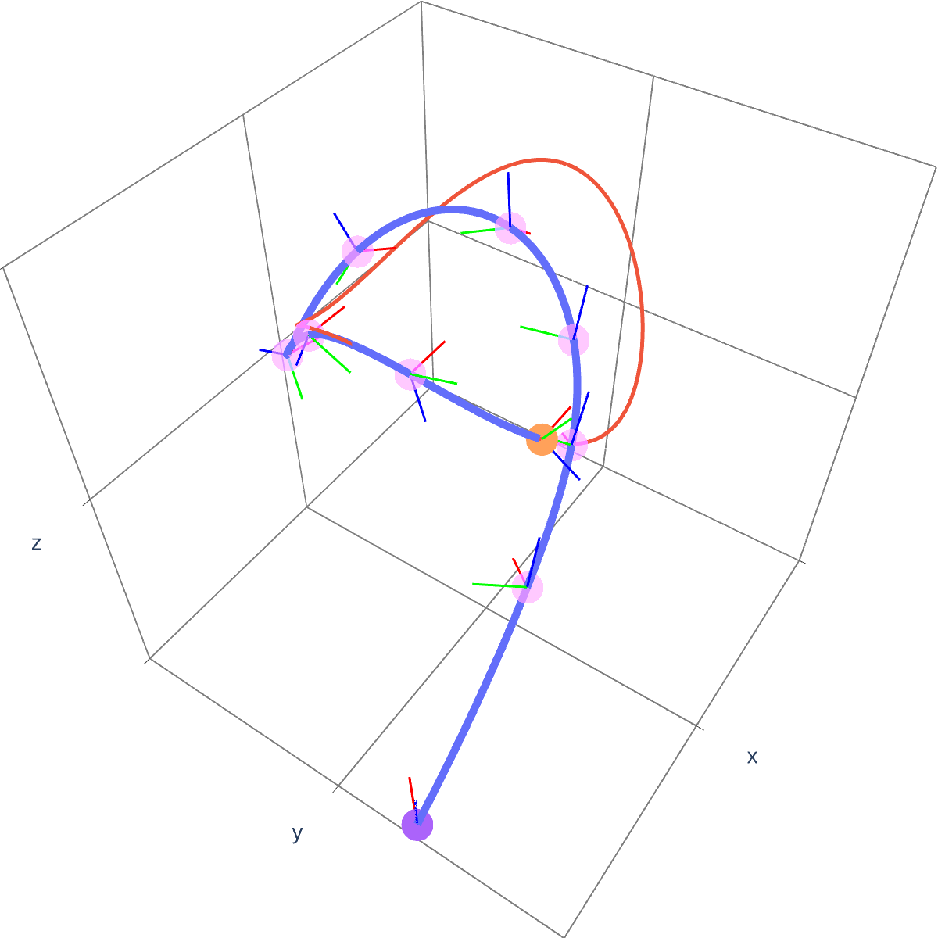
\includegraphics[width=\textwidth]{figures/vf_automatica_1.pdf} % Replace with your image
        \caption{$t\in[0, 5]s$}
        \label{fig:vfplot-first}
    \end{subfigure}
    \hfill
    % Second subfigure
    \begin{subfigure}[b]{0.32\textwidth}
        \centering
        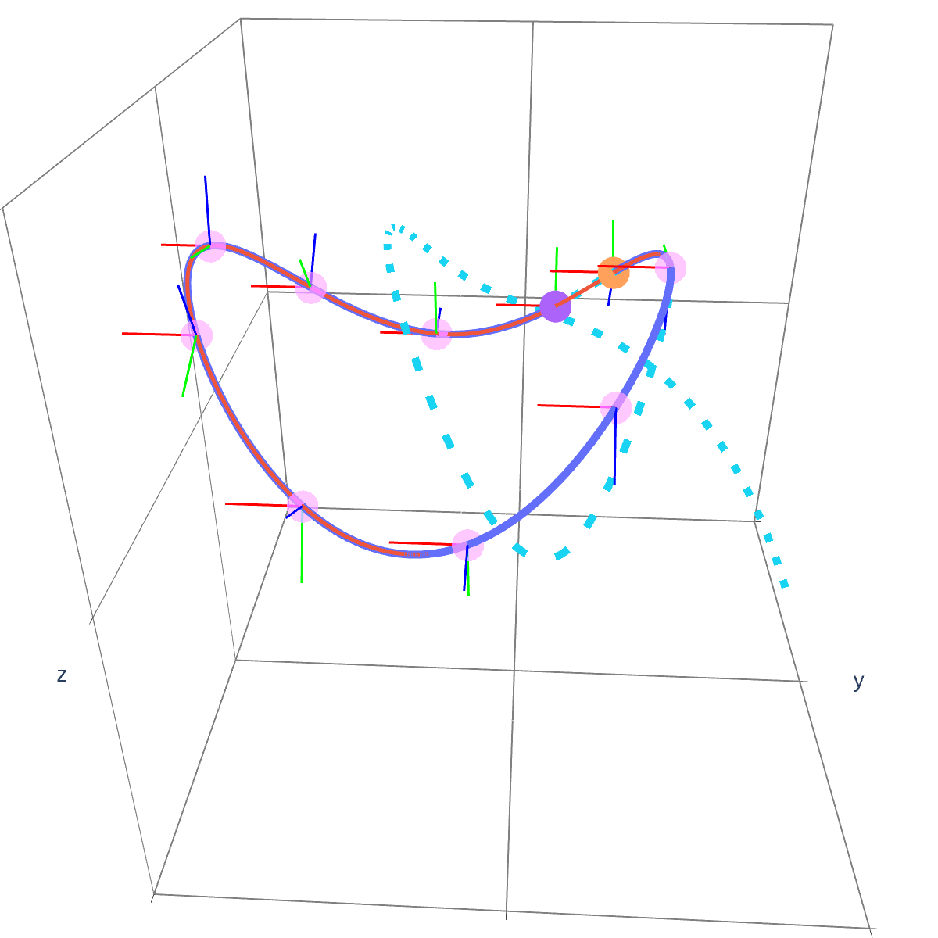
\includegraphics[width=\textwidth]{figures/vf_automatica_2.pdf} % Replace with your image
        \caption{$t\in[5, 9.7]s$}
        \label{fig:vfplot-second}
    \end{subfigure}
    \hfill
    % Third subfigure
    \begin{subfigure}[b]{0.32\textwidth}
        \centering
        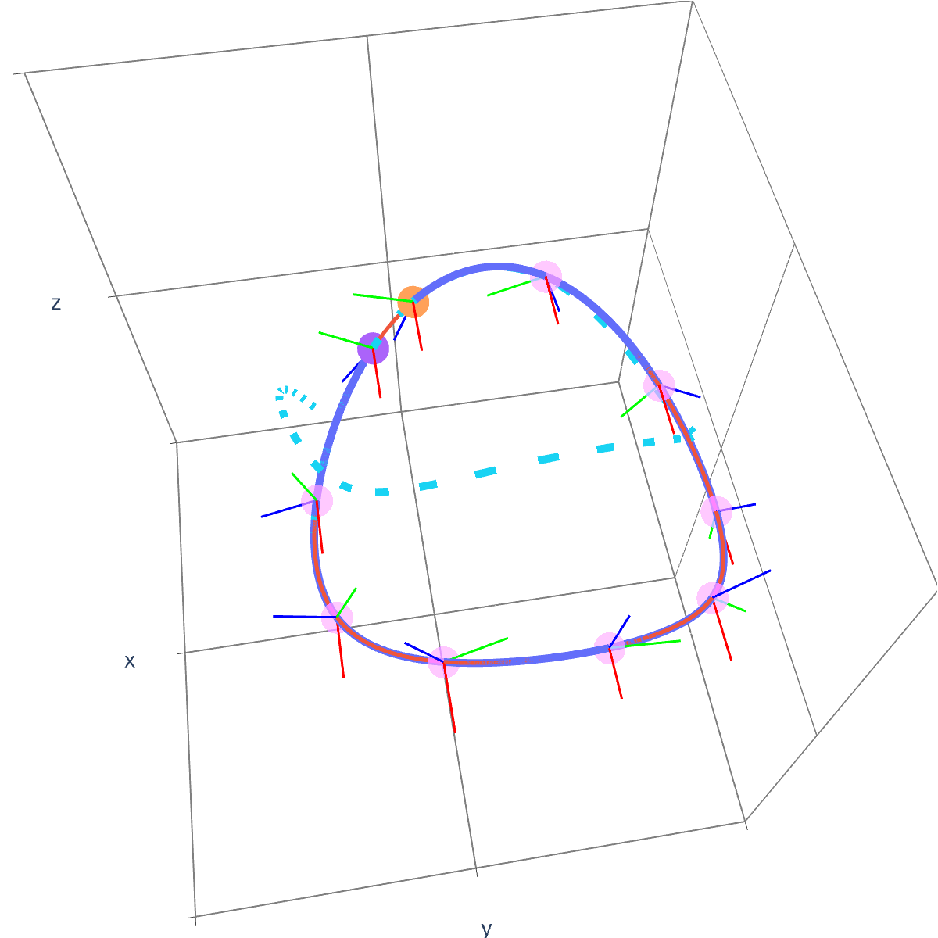
\includegraphics[width=\textwidth]{figures/vf_automatica_3.pdf} % Replace with your image
        \caption{$t\in[9.7, 14.5]s$}
        \label{fig:vfplot-third}
    \end{subfigure}
    \caption{The solid blue line depicts the system trajectory, while the solid red line indicates the target curve. The dashed light blue line represents the past trajectory. The initial and final positions are marked by purple and orange spheres, respectively. Translucent pink spheres denote intermediary positions, with orientation frames shown by RGB axes.}
    \label{fig:vfplot-trajectory}
\end{figure}
\begin{figure}[ht!]
    \centering
    \def\svgwidth{.8\linewidth}
    {\tiny\import{figures/}{distance_pos_ori_D.pdf_tex}}
    \caption{Value of EC-distance $D$, position error in centimeters and orientation error in degrees along time.}
    \label{fig:position-orientation-errors}
\end{figure}
We implemented the code in C++. On average, the computation of the vector field took $60\pm5$ milliseconds per iteration on a single core of an Intel i5-10300H @ 4.5GHz CPU, with 8 GB of RAM. On average, $99.5\%$ of this time was spent solving the optimization problem in \eqref{eq:optimization-problem-distance-definition-point-curve}. Since the optimization process is highly parallelizable -- allowing for the simultaneous computation of $\widehat{D}(\mathbf{H},\mathbf{H}_d(s))$ across different discretized $s$ -- the computational effort could be significantly reduced by leveraging parallel architectures such as GPUs, SIMD, or multi-threading. The system's trajectory is illustrated in \cref{fig:vfplot-trajectory}, while the values of the distance function $D$ are shown in \cref{fig:position-orientation-errors}. Additionally, \cref{fig:position-orientation-errors} provides a more intuitive representation of the position error (in centimeters) and the orientation error (in degrees). The results confirm that the system successfully converges to the desired curve and circulates around it as expected. Once the system reaches the curve, it remains there without deviation. Although our implementation was carried out in C++, we provide a less efficient sample code in Python for clarity and accessibility, available at \url{https://github.com/fbartelt/SE3-example/blob/main/SE3example.ipynb}.